\documentclass{article}
\usepackage[T1]{fontenc}
\usepackage[utf8]{inputenc}

\usepackage{cmbright}
\usepackage[T1]{fontenc}

\usepackage{multicol}

\usepackage{amsmath}
\usepackage{amsfonts}
\usepackage{amssymb}
\usepackage{tikz}
\usepackage{graphicx}
\graphicspath{  {./images/} }
\setlength{\parindent}{0pt}
\usepackage{changepage}
\usepackage{verbatim}
\usepackage{physics}
\usepackage{derivative}
\usepackage{bm}
\usepackage[colorlinks=true, linkcolor=blue, urlcolor=blue, citecolor=blue, anchorcolor=blue]{hyperref}

\addtolength{\oddsidemargin}{-.25in}
\addtolength{\textwidth}{0.5in}

\makeatletter
\newcommand*\bigcdot{\mathpalette\bigcdot@{.5}}
\newcommand*\bigcdot@[2]{\mathbin{\vcenter{\hbox{\scalebox{#2}{$\m@th#1\bullet$}}}}}
\makeatother

\DeclareMathOperator{\di}{d\!}
\newcommand*\Eval[3]{\left.#1\right\rvert_{#2}^{#3}}

\newcommand{\uvec}[1]{\boldsymbol{\hat{\textbf{#1}}}}
\newcommand{\vr}[1]{\textbf{#1}}

\newcommand{\thus}[0]{\; \; \longrightarrow \; \;}

\newcommand{\lag}{\mathcal{L}}
\newcommand{\ham}{\mathcal{H}}

\title{Sky Location Calculations}
\author{Ryan Liu}
\date{Last updated: July 25, 2021}

\begin{document}

\maketitle

\section{Resources Used}

\begin{itemize}
    \item B Schutz. \textit{Networks of gravitational wave detectors and three figures of merit}. \url{https://arxiv.org/abs/1102.5421}
    \item M Dominik et al. \textit{Double Compact Objects. III. Gravitational-Wave Detection Rates}. \url{https://iopscience.iop.org/article/10.1088/0004-637X/806/2/263}
    \item Chen et al. \textit{Distance Measures in gravitational-wave astrophysics and cosmology.} \url{https://arxiv.org/abs/1709.08079}
    \item Belczynski et al. \textit{Compact binary merger rates: Comparison with LIGO/VIRGO upper limits}. \url{https://arxiv.org/abs/1510.04615}
\end{itemize}

\section{Notes}

Suppose that a detector is located with arms in the $xy$-plane, and that the location of the source of a gravitational wave is denoted by the spherical coordinates $\theta$ and $\phi$. It follows that the detected strain is 
\begin{equation}
    \frac{\delta L(t)}{L} = F_+ (\theta, \phi, \psi) h_+ (t) + F_{\cross} (\theta, \phi, \psi) h_{\cross} (t)
\end{equation}
where $h_+(t)$ and $h_{\cross} (t)$ are the polarizations of the GW (rotated at an angle $\psi$ relative to the detector axes) and $F_+$ and $F_{\cross}$ are the antenna pattern functions given by 
\begin{gather}
    F_+ = \frac{1}{2} (1 + \cos^2 \theta) \cos 2 \phi \cos 2 \psi - \cos \theta \sin 2 \phi \sin 2 \psi \\
    F_{\cross} = \frac{1}{2} (1 + \cos^2 \theta) \cos 2 \phi \sin 2 \psi + \cos \theta \sin 2 \phi \cos 2 \psi
\end{gather}
We find that the expectation value of the SNR is 
\begin{equation}
    \langle \rho^2 \rangle = 2 \Big[ F_+^2 + F_{\cross}^2 \Big] \int_0^\infty \frac{\abs{H(f)}^2}{S_h (f)} df
\end{equation}
where $\abs{H(f)}^2 = \abs{H_+}^2 + \abs{H_{\cross}}^2$. At the optimal location, namely $\theta = 0$ or $\pi$ ($\phi$ has no effect here and $\psi$ is averaged over), we find that 
\begin{equation}
    P(\theta=0, \phi) = \Big[ F_+^2(\theta=0, \phi, \psi) + F_{\cross}^2 (\theta=0, \phi, \psi) \Big] = 1
\end{equation}
Otherwise, the SNR is weaker by a factor of 
\begin{equation}
    P(\theta, \phi) = \frac{1}{4} (1 + \cos^2 \theta)^2 \cos^2 2 \phi + \cos ^2 \theta \sin^2 2 \phi
\end{equation}
Therefore, relative to the optimally-positioned GW signal, an arbitrarily located signal must be stronger by a factor of $P(\theta, \phi)^{-1}$. \\

It is also possible to approximate the reduction in BBH merger detections by considering the ratio between the antenna volume and comoving volume at a particular redshift. Suppose that the GW signal is oriented at sky location $\Omega$ with polarization $\psi$ and inclination $\iota$, and that the projection parameter (equivalent to $P(\theta, \phi)$ above) is denoted by $w$. Then, the cumulative distribution function of $w$ is given by
\begin{equation}
    P(w) = \int_V \frac{d \Omega}{4 \pi} \frac{d \psi}{\pi} \frac{d \cos \iota}{2}
\end{equation}
Based on a Monte Carlo simulation of $10^9$ binaries, an analytic approximation for this distribution is
\begin{equation}
    p_{det}(w) =a_2(1-w/\alpha)^2 + a_4(1-w/\alpha)^4 + a_8(1-w/\alpha)^8 + (1-a_2-a_4-a_8)(1-w/\alpha)^{10}
\end{equation}
where 
\begin{equation}
    a_2 = 0.374222, \quad a_4 = 2.04216, \quad a_8 = -2.63948, \quad \alpha = 1.0
\end{equation}
It follows that for a given merger with corresponding maximum redshift of detection (horizon redshift) $z_{hor}$, the antenna volume is
\begin{equation}
    V_{antenna} = 4 \pi \int_0^{z_{hor}} \frac{1}{1+z} \frac{dV_c}{dz} p_{det} \Big( \frac{D_L(z)}{D_L(z_{hor})} \Big) dz 
\end{equation}
A simplified approximation for low redshifts (iLIGO detection range, $z < 1$) is given by 
\begin{equation}
    V_{antenna} \approx \frac{V_{tot}}{(2.264)^3} = \frac{V_{tot}}{11.605}
\end{equation}

\section{SNR Approximation}

In order to quickly approximate the effect of distance/redshift on the SNR of a GW signal, we find an analytic function that takes the computed SNR of a signal at an arbitrary redshift, and outputs the approximate SNR at the desired redshift. By visual approximation, we find that such a function is 
\begin{equation}
    \rho(m, z) = \frac{\rho_0 D_0}{D_L(z)} \Big[ \Big(\frac{z \sqrt{m}}{50} \Big)^{\sqrt{m}} + \Big( \frac{z \sqrt{m}}{50} \Big) + 1 \Big]^{-1}
\end{equation}
where $\rho_0$ and $D_0$ are the computed SNR and luminosity distance respectively, and $D_L(z)$ is the luminosity distance at the desired redshift $z$. Similarly, given a desired SNR the desired luminosity distance can be found through parameter estimation. Evidently, this approximation assumes that $m=m_1=m_2$ and that the black holes have 0 spin. \\

\begin{figure}[!htb]
    \center{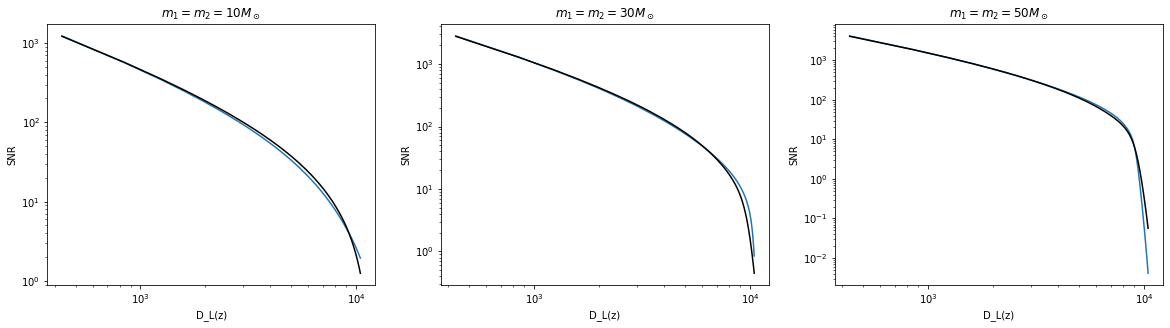
\includegraphics[width=\textwidth]{SNR41.png}}
    \caption{\label{fig:approx} Actual (blue) and approximated (black) SNR of several GW signals assuming zero spin and optimal sky location, using Cosmic Explorer design sensitivity.}
\end{figure}

Visually, we can see that this approximation maintains very high accuracy, especially for predcting lumonisty distance based on SNR, for all but extreme SNR or $D_L$ values. 

\section{Results}

We first compare the effective antenna volume to the total volume over the full redshift spectrum, using the approximation from Eq. (8) and (9). We notice from Fig. \ref{fig:antenna} that for low redshifts, there is strong agreement between the Euclidean approximation from Eq. (11); however, at high redshifts, the actual effective antenna volume is approximately 30\% - 40\% larger, in agreement with comments from Belczynski et al. 

\begin{figure}[!htb]
    \center{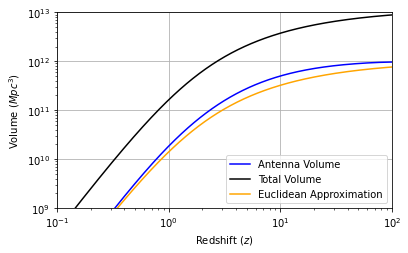
\includegraphics[width=3.25in]{SNR42.png}}
    \caption{\label{fig:antenna} Comoving volume and antenna volume at various redshifts}
\end{figure}

We now consider the effect of sky location on the strength of a GW signal. Using Eq. (6), we see from Fig. \ref{fig:spherical} that the polar and azimuthal angle changes follow a 90 degree cycle, as expected. It is clear that there will be a significant reduction in signal detection for a majority un-optimally located mergers. If visualized in three-dimensions, this figure replicates the ``peanut-shaped" antenna pattern as illustrated in Fig. 2 of Schutz. We note that \textbf{this does not take into account inclination angle}, which will further reduce signal strength for all $\iota \neq 0$. 

\begin{figure}[!htb]
    \center{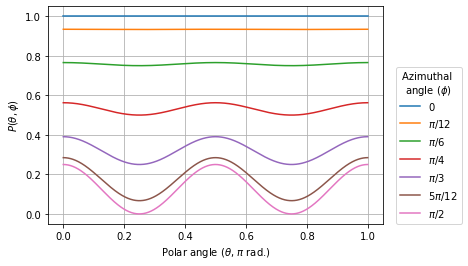
\includegraphics[width=3.5in]{SNR43.png}}
    \caption{\label{fig:spherical} Relative strength of an arbitrary GW at various sky locations $(\theta, \phi)$}
\end{figure}

As mergers are assumed to be uniformly distributed with respect to sky location, we create bins of radial ``cones" that contain an equal proportion of the total mergers to approximate at what radial distance mergers in different parts of the sky can be detected. A random distribution in spherical coordinates is given by selecting random points along the distribution of $\cos \theta$ and $\phi$. 

\begin{figure}[!htb]
    \center{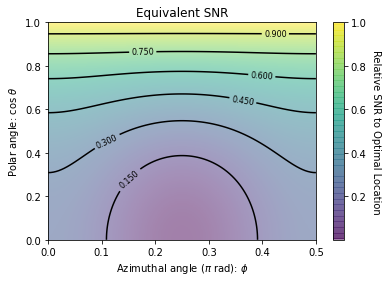
\includegraphics[width=2.6in]{SNR44.png} 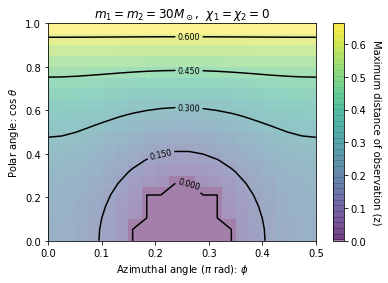
\includegraphics[width=2.6in]{SNR45.png}}
    \caption{\label{fig:distance} (Left) $P(\theta, \phi)$ over the first octant. (Right) Maximum redshift of detection for a $m_1 = m_2 = 30 M_\odot$ BBH merger at aLIGO design sensitivity, calculated over 20 equally spaced bins of $\phi$ and $\cos \theta$ each; $z < 0.1$ is denoted as $z=0$.}
\end{figure}

We find from Fig. \ref{fig:distance} that the maximum horizon redshift for a $m_1=m_2=30 M_\odot$ merger is $z \approx 0.663$, whereas the mean horizon redshift over all sky locations is $z \approx 0.305$, a reduction factor of $2.170$. This is in close agreement with the iLIGO approximation of Eq. (11) and the polynomial approximation of Eq. (8). However, because merger rates are not uniform throughout the entire antenna volume, it will be more accurate to calculate the expected number of detections individually for each bin rather than dividing the total number of mergers within the maximum horizon redshift by the reduction factor. 

\end{document}